\subsection{Построение бифуркационной диаграммы}
            
\begin{definition}
        Динамическая система~$u \mapsto f(u)$ называется топологически эквивалентной в области $U \subseteq X$ динамической системе~$v \mapsto g(v)$ в областе $V \subseteq X$, если существует гомеоморфизм $h:X\rightarrow X,\; h(U) = V$, отображающий орбиты первой системы в $U$ на орбиты второй системы в $V$, сохраняя ориентацию во времени. \cite[стр.~396]{bratus10}
\end{definition}
\textit{Замечание.} Фазовые портреты эквивалентных систем также называются топологически эквивалентными.

\begin{definition}
        Появление топологически неэквивалентных фазовых портретов при изменении параметров динамической системы называется бифуркацией. \cite[стр.~25]{bratus10}
\end{definition}
\textit{Замечание.} Таким образом, бифуркация~--- это изменение топологического типа системы, когда параметры проходят через некоторые \textit{бифуркационные (критические)} значения. \cite[стр.~25]{bratus10}

\begin{definition}
        Бифуркационной диаграммой динамической системы называется разбиение пространства параметров на максимальные связные подмножества, которые определяются соотношениями топологической эквивалентности и рассматриваются вместе с фазовыми портретами для каждого элемента разбиения. \cite[стр.~27]{bratus10}
\end{definition}

Бифуркационная диаграмма одномерной динамической системы с одним параметром~$r$ может быть представлена на плоскости~$(u, r)$. Фазовые портреты в данном случае~--- это сечения бифуркационной диаграммы при $r = const$.

Рассмотрим алгоритм построения бифуркационной диаграммы:
\begin{enumerate}
        \item Возьмем достаточно мелкое разбиение (выбран шаг $\Delta_r = 0.01$) выбранного отрезка параметра~$r$.
        \item Для каждого значения параметра из разбиения:
        \begin{enumerate}
                \item Прогоним первые $n$ (взято $n = 1000$) значений $u_t$ системы при некотором $u_0$ (взято $u_0 = 4$), чтобы траектория сошлась к некоторому \textit{постоянному} состоянию, например, предельной точке или циклу (определение цикла будет дано позднее).
                \item Посчитаем следующие $m$ (взято $m = 100$) значений $u_t$, которые и будут зафиксированны (изображены на координатной плоскости как точки $(r, u_t)$) как фазовые портреты при фиксированных значениях параметра $r$.
        \end{enumerate}
        \item Изобразив полученные $m$ точек на плоскости для каждого значения параметра из разбиения, получим бифуркационную диаграмму системы.
\end{enumerate}

\begin{figure}[h]
        \centering
        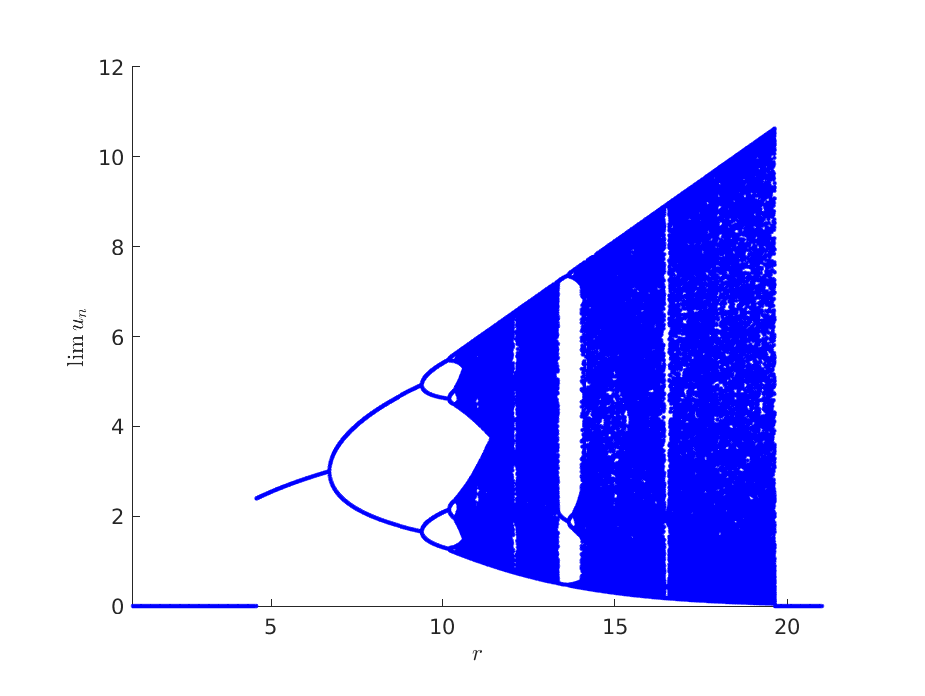
\includegraphics[width=0.8\linewidth]{img/one_step_bifurcation.eps}
        \caption{Бифуркационная диаграмма для системы \ref{eq:first_discrete_system}. Начальное приближение $u_0 = 4$. $1 \leqslant r \leqslant 21$.}
        \label{img:one_step_bifurcation}
\end{figure}